\documentclass{beamer}
\usetheme{Boadilla}
\usepackage{bibentry}
\usepackage{cmbright}
\usepackage{natbib}
\setbeamertemplate{itemize items}[circle]
\setbeamertemplate{enumerate items}[default]

\def\E{\text{E}}
\def\Var{\text{Var}}
\def\Cov{\text{Cov}}

\title[Euler Equation]{Work in Progress: The Euler Equation Implied Rate Under Heterogeneous Preferences}
\author[Li]{Pearl Li}
\date{February 3, 2016}

\begin{document}

\begin{frame}
\titlepage
\end{frame}


\begin{frame}{Last Time}
\begin{itemize}
\item Literature review
\item Cleaned raw data from FRED
\item Estimated VAR(4) for consumption, inflation, leisure, FFR, ...
\item Computed implied interest rates under CRRA utility
  \begin{itemize}
  \item Implied real rates corresponded well to \cite{collard11}
  \item Implied nominal rates were very bad...
  \end{itemize}
\end{itemize}
\end{frame}

\begin{frame}{Last Time}
\begin{center}
\begin{tabular}{cc}
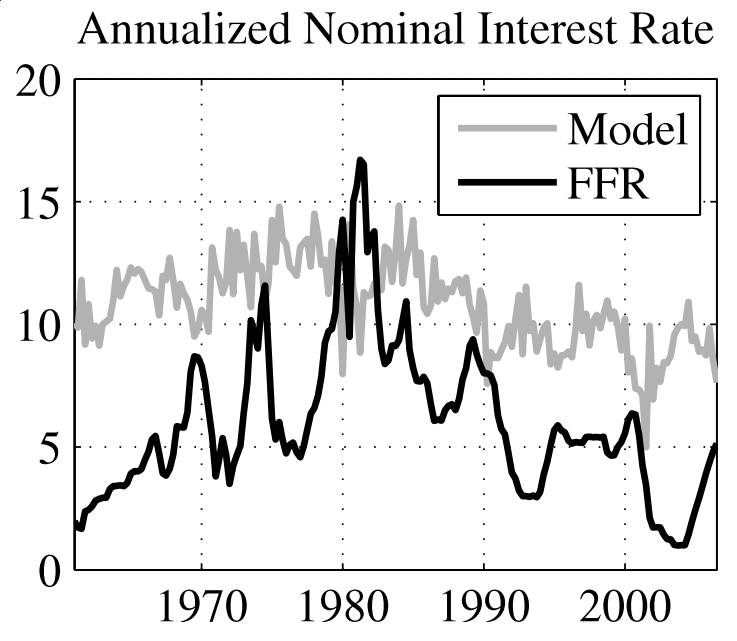
\includegraphics[height=120px]{figs/old/crra-nominal_collard.png} &
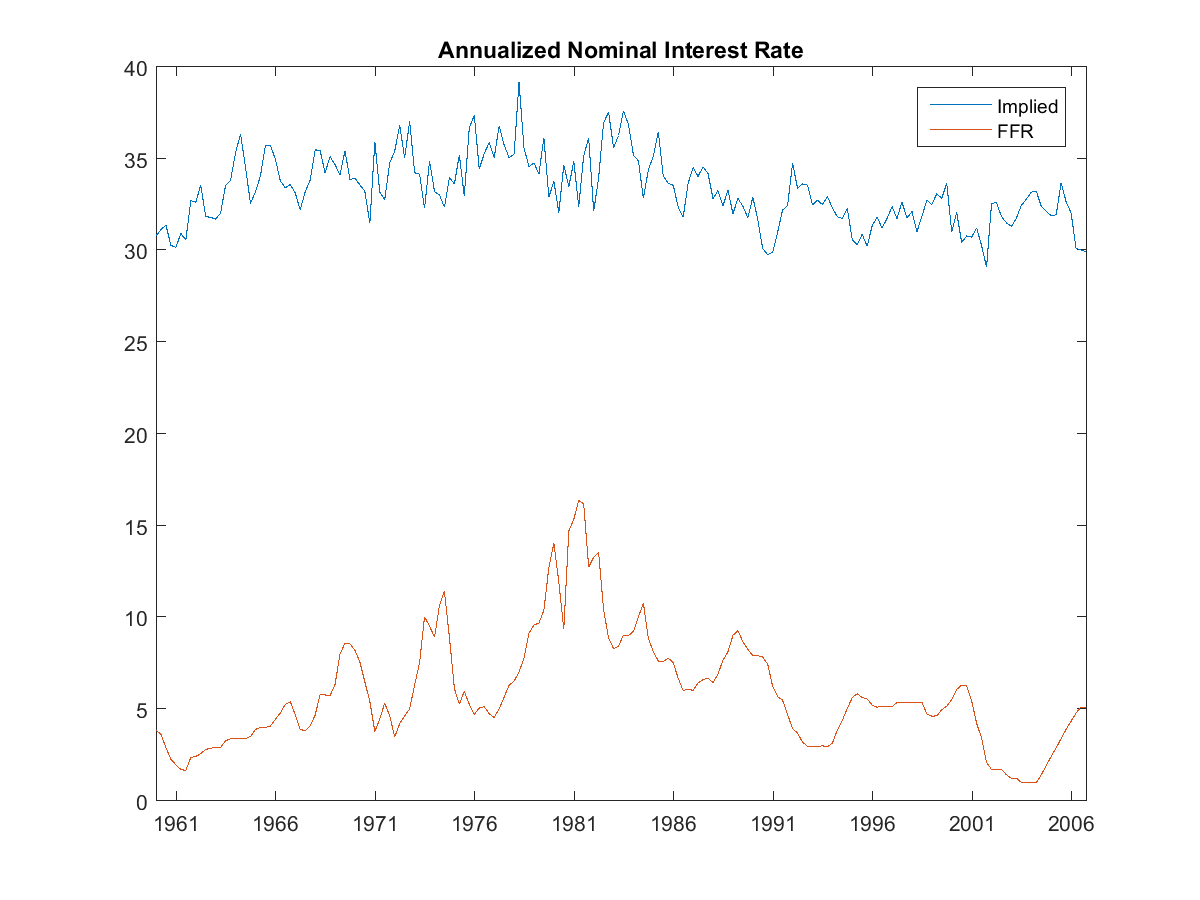
\includegraphics[height=120px]{figs/old/crra-nominal.png} \\
\cite{collard11} & Li (2015)
\end{tabular}
\end{center}
\begin{itemize}
\item It turns out this resulted from a matrix indexing error
\end{itemize}
\end{frame}

\begin{frame}{Generalized Implied Rates}
\begin{itemize}
\item As in \cite{collard11}: $$u(C_t, \ell_t) = \frac{[(C_t/C_{t-1}^\varphi)^\nu \ell_t^{1-\nu}]^{1-\alpha}}{1-\alpha}$$
\item Discount factor $\beta = 0.9926$
\item Coefficient of risk aversion $\alpha = 2$
\item \textbf{Habit persistence parameter $\varphi = 0.8$}
\item \textbf{Weight assigned to consumption $\nu = 0.34$}
\item When $\varphi = 0$ and $\nu = 1$, this reduces to CRRA utility (last time)
\end{itemize}
\end{frame}

\begin{frame}{Generalized Implied Rates}
\begin{itemize}
\item Euler equation (from first-order conditions)
  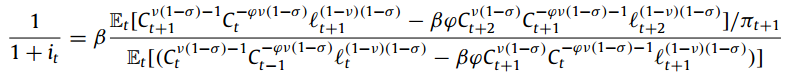
\includegraphics[width=0.9\textwidth]{figs/euler-equation.png}
\item Assuming conditional lognormality, nominal interest rate given by
$$\frac{1}{1+i_t} = \beta \frac{\exp(\chi_{1t}) - \beta \varphi \exp(\chi_{2t})}{\exp(\chi_{3t}) - \beta \varphi \exp(\chi_{4t})}$$
\begin{align*}
\chi_{1t} &= (\nu(1-\alpha)-1) \E_t c_{t+1} - \varphi\nu(1-\alpha)c_t + (1-\nu)(1-\alpha) \E_t \ell_{t+1} \\
  &\qquad - \E_t \pi_{t+1} + \text{constant second-order moments} \\
\chi_{2t} &= \ldots
\end{align*}
\item Real interest rate is same without inflation terms
\end{itemize}
\end{frame}

\begin{frame}{Treatments}
$$u(C_t, \ell_t) = \frac{[(C_t/C_{t-1}^\varphi)^\nu \ell_t^{1-\nu}]^{1-\alpha}}{1-\alpha}$$
\bigskip
\begin{center}
\begin{tabular}{|l|c|c|p{0.5\textwidth}|} \hline
& $\phi$ & $\nu$ & Specification \\ \hline
SEP & 0 & 1 & CRRA \\
SEP + HP & 0.8 & 1 & habit persistence \\
NSEP & 0 & 0.34 & nonseparable consumption and leisure \\
NSEP + HP & 0.8 & 0.34 & nonseparable consumption and leisure + habit persistence \\ \hline
\end{tabular}
\end{center}
\end{frame}

\begin{frame}{Results: SEP}
\begin{center}
\begin{tabular}{cc}
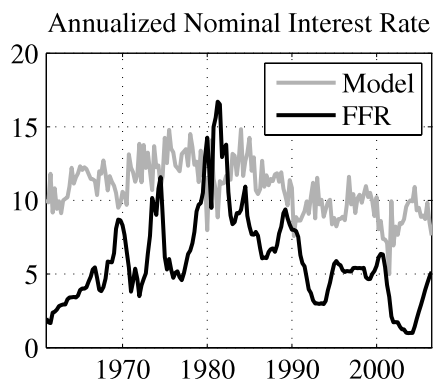
\includegraphics[height=90px]{figs/implied_ffr/nominal_1_collard.png} &
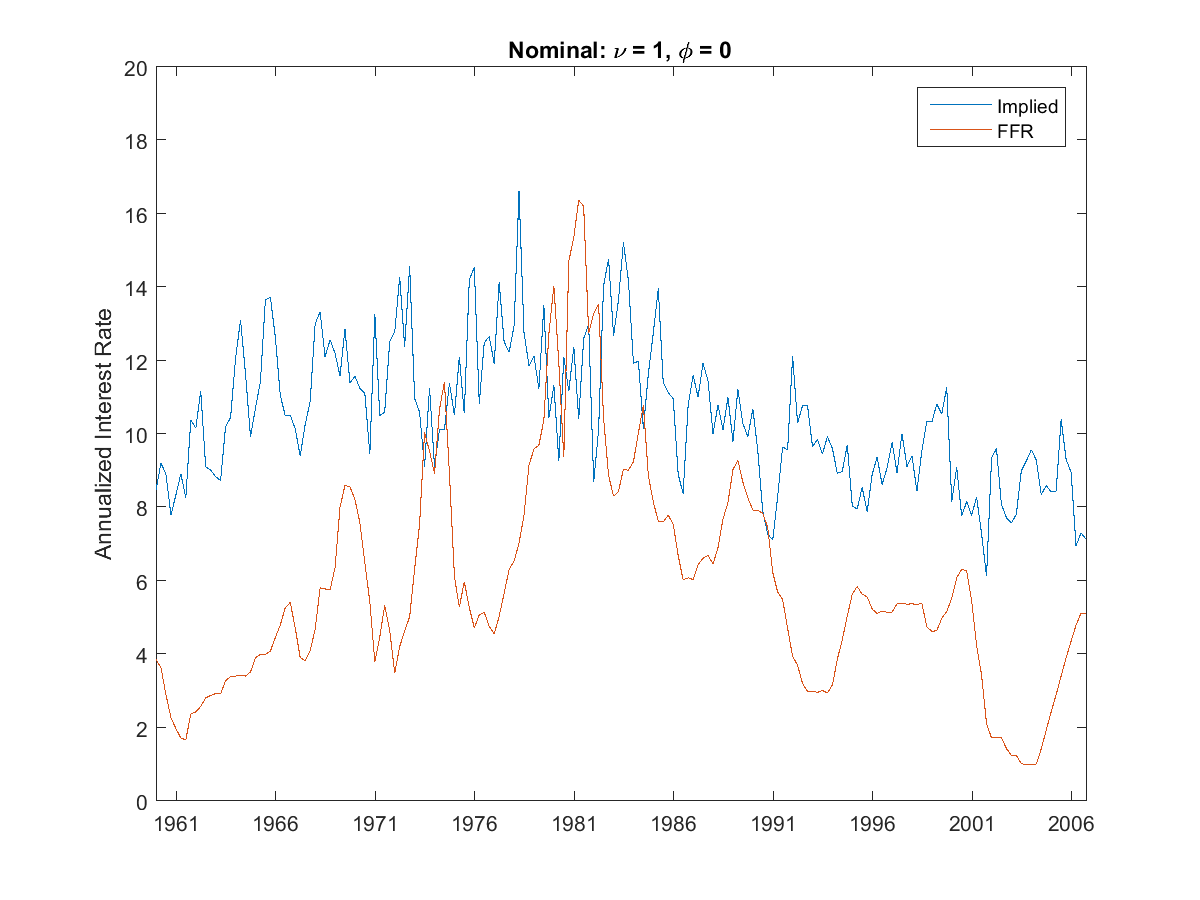
\includegraphics[height=90px]{figs/implied_ffr/nominal_1.png} \\
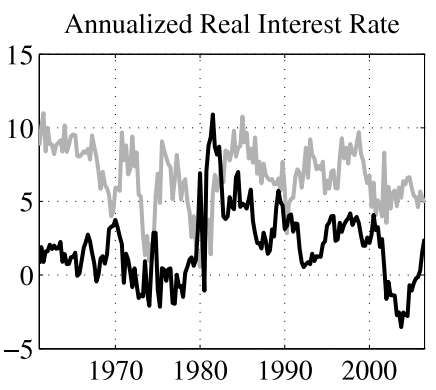
\includegraphics[height=90px]{figs/implied_ffr/real_1_collard.png} &
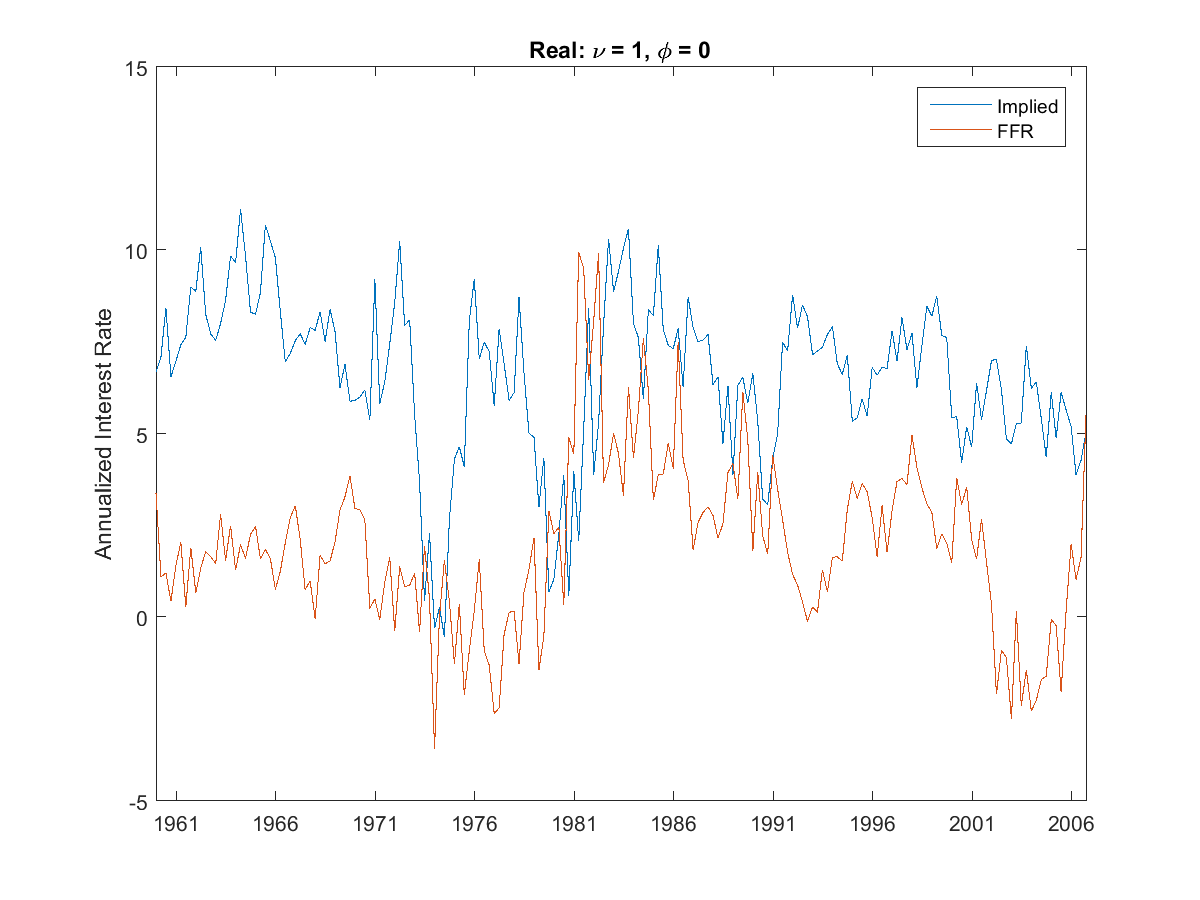
\includegraphics[height=90px]{figs/implied_ffr/real_1.png} \\
\cite{collard11} & Li (2016)
\end{tabular}
\end{center}
\end{frame}

\begin{frame}<1>[label=implied_ffr_sep-hp]
  \frametitle<1>{Results: SEP + HP}
  \frametitle<2>{Problems: SEP + HP Implied Rates}
\begin{center}
\begin{tabular}{cc}
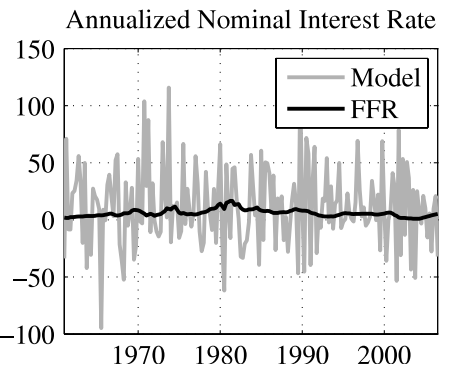
\includegraphics[height=90px]{figs/implied_ffr/nominal_2_collard.png} &
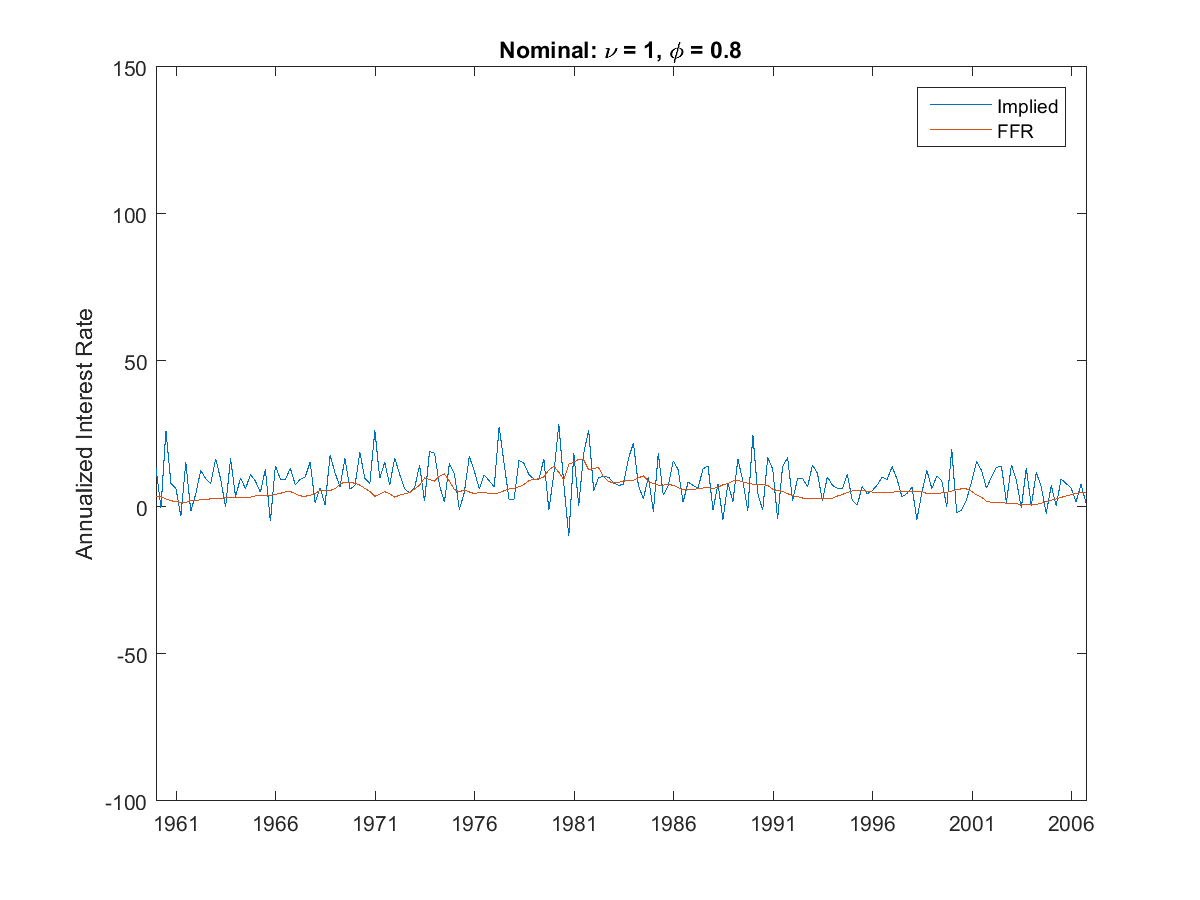
\includegraphics[height=90px]{figs/implied_ffr/nominal_2.png} \\
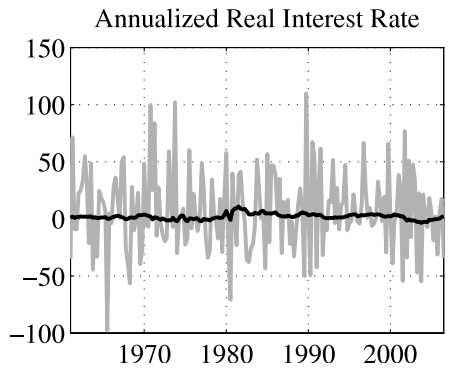
\includegraphics[height=90px]{figs/implied_ffr/real_2_collard.png} &
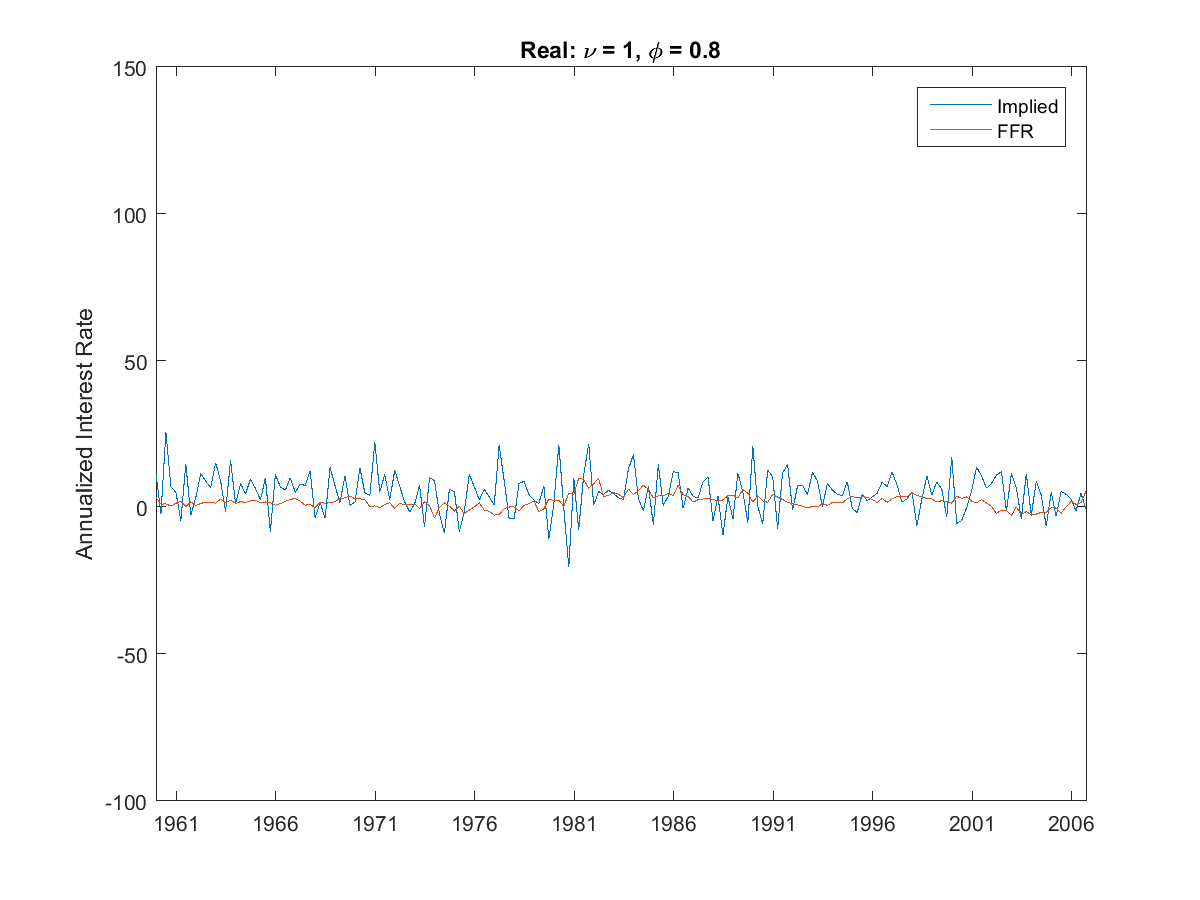
\includegraphics[height=90px]{figs/implied_ffr/real_2.png} \\
\cite{collard11} & Li (2016)
\end{tabular}
\end{center}
\end{frame}

\begin{frame}{Results: NSEP}
\begin{center}
\begin{tabular}{cc}
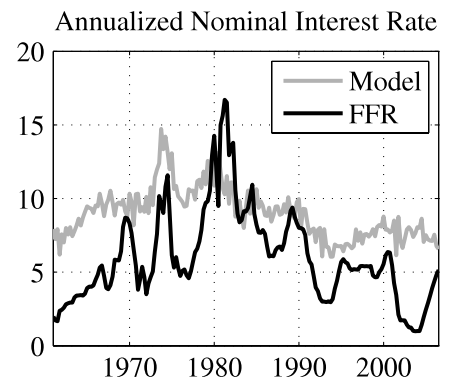
\includegraphics[height=90px]{figs/implied_ffr/nominal_3_collard.png} &
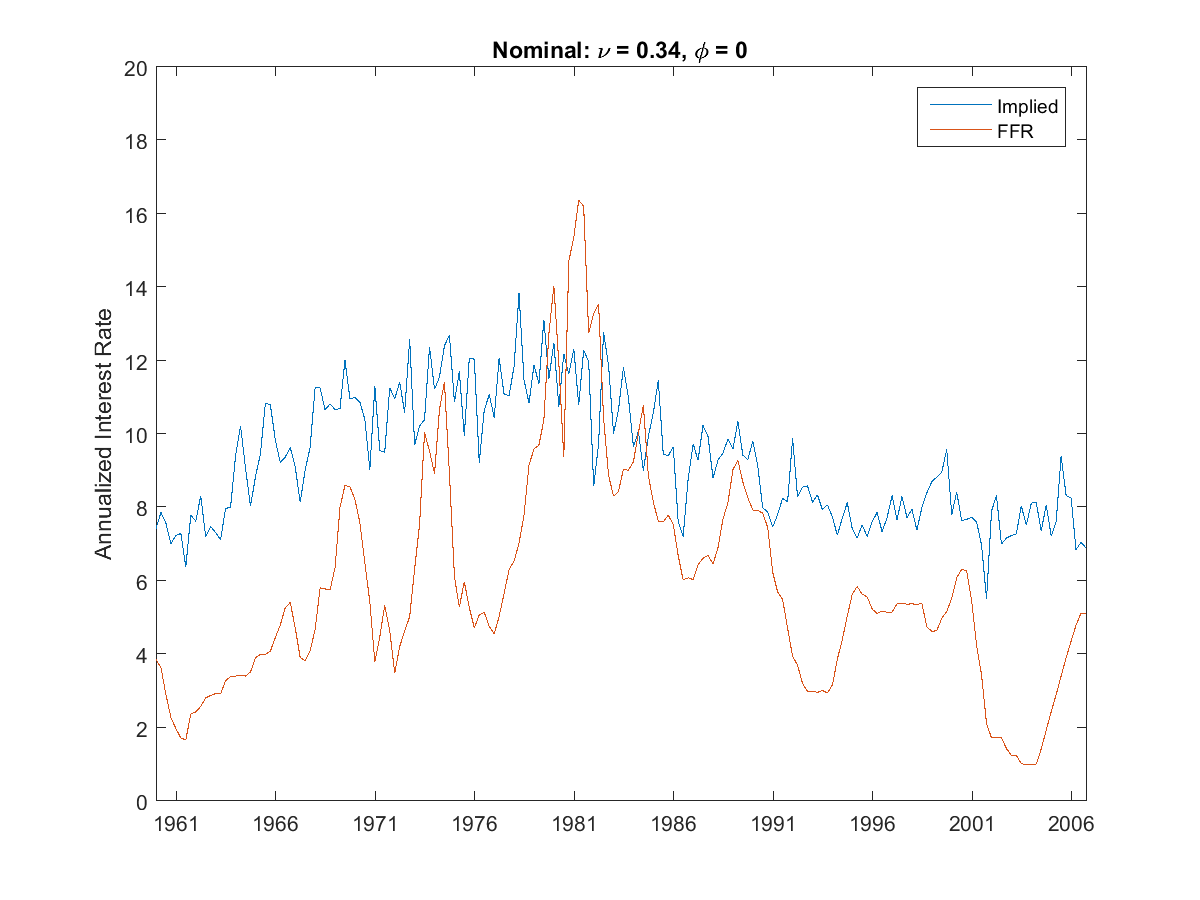
\includegraphics[height=90px]{figs/implied_ffr/nominal_3.png} \\
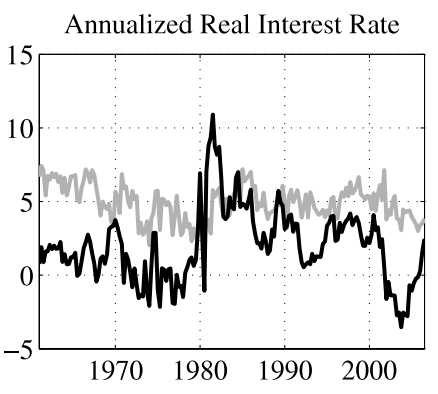
\includegraphics[height=90px]{figs/implied_ffr/real_3_collard.png} &
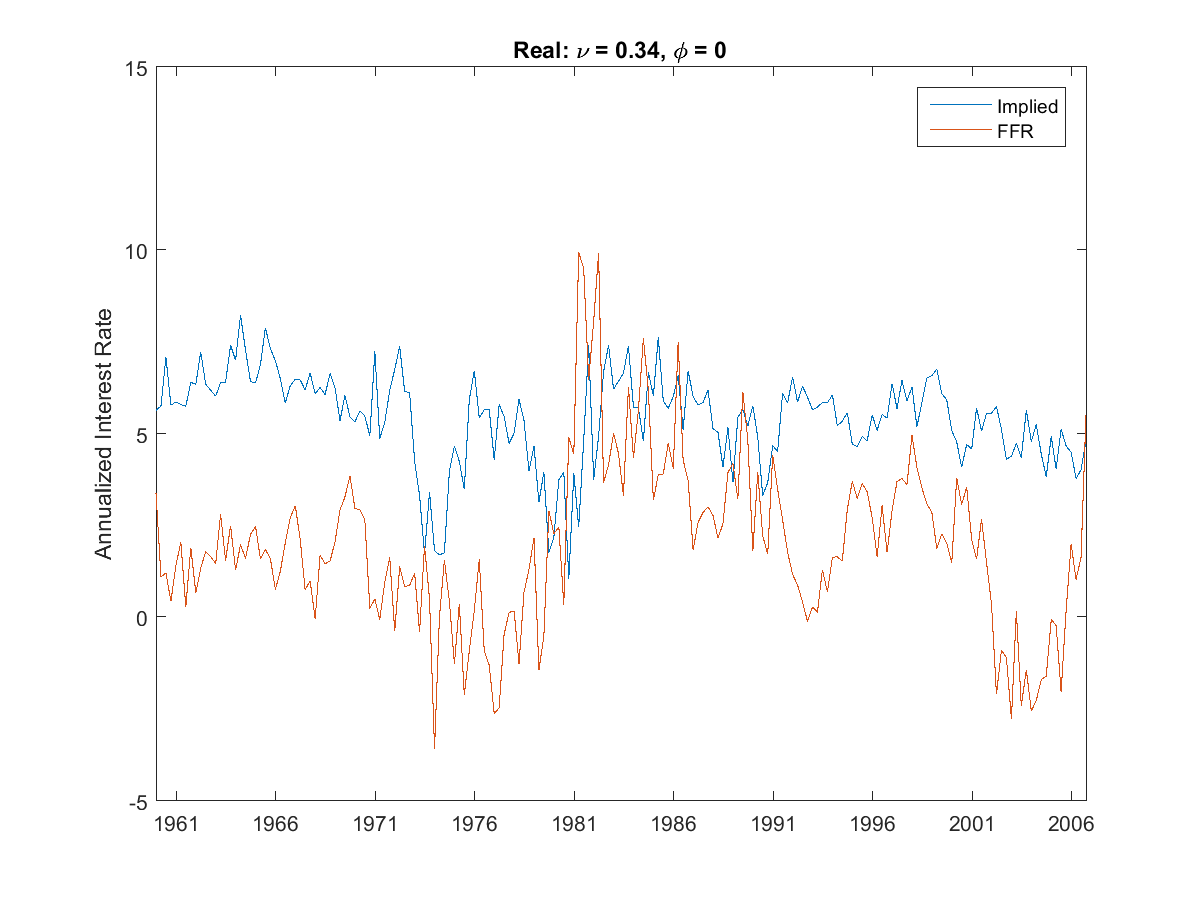
\includegraphics[height=90px]{figs/implied_ffr/real_3.png} \\
\cite{collard11} & Li (2016)
\end{tabular}
\end{center}
\end{frame}

\begin{frame}{Results: NSEP + HP}
\begin{center}
\begin{tabular}{cc}
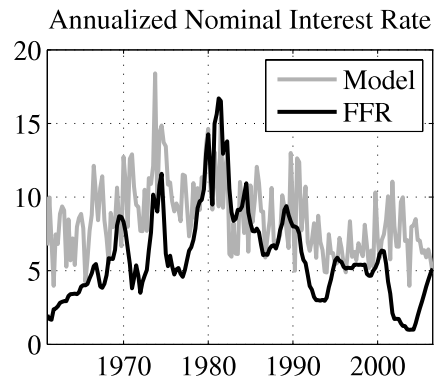
\includegraphics[height=90px]{figs/implied_ffr/nominal_4_collard.png} &
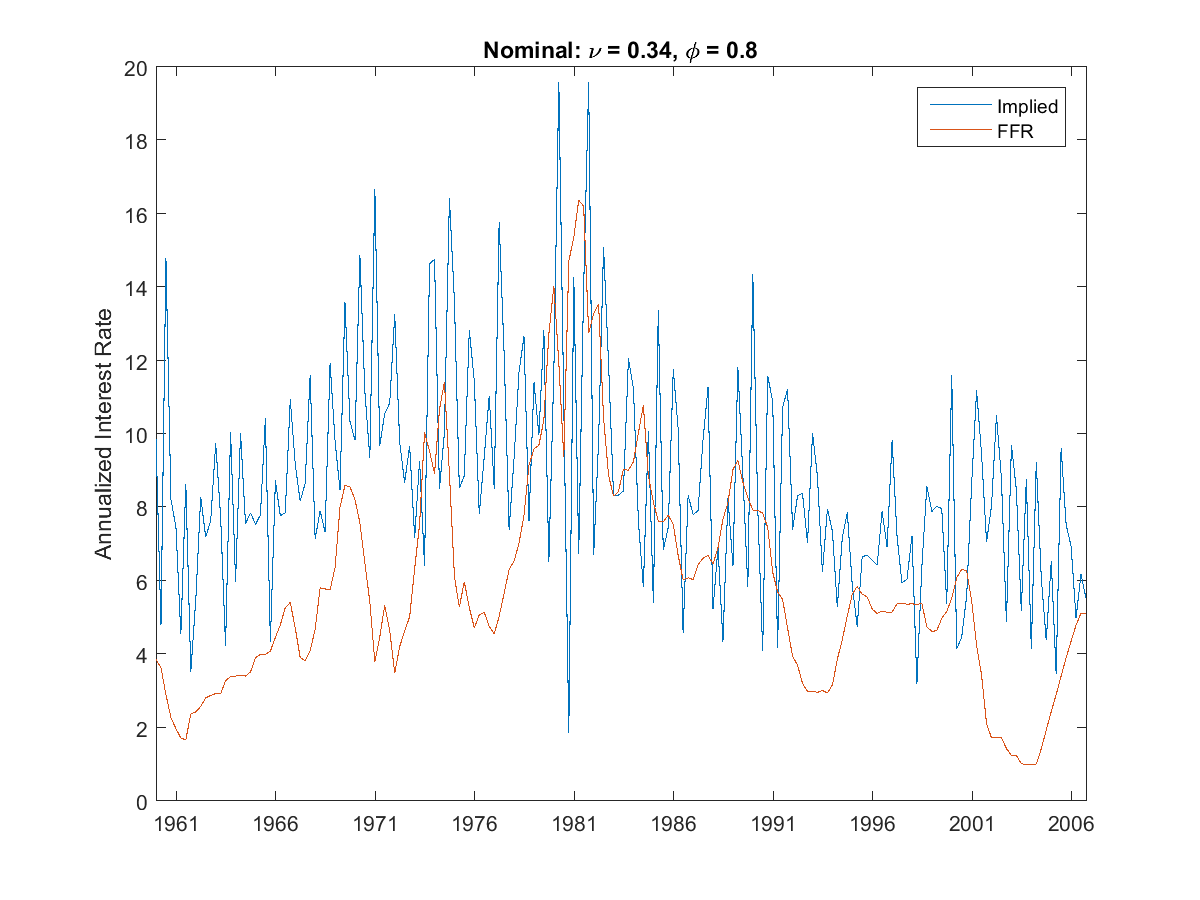
\includegraphics[height=90px]{figs/implied_ffr/nominal_4.png} \\
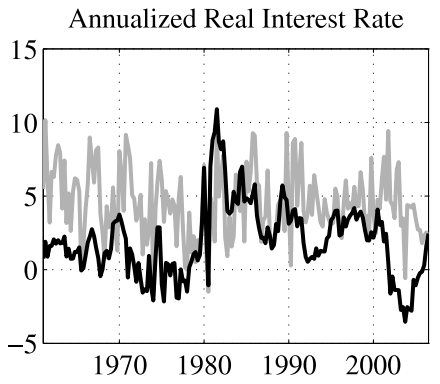
\includegraphics[height=90px]{figs/implied_ffr/real_4_collard.png} &
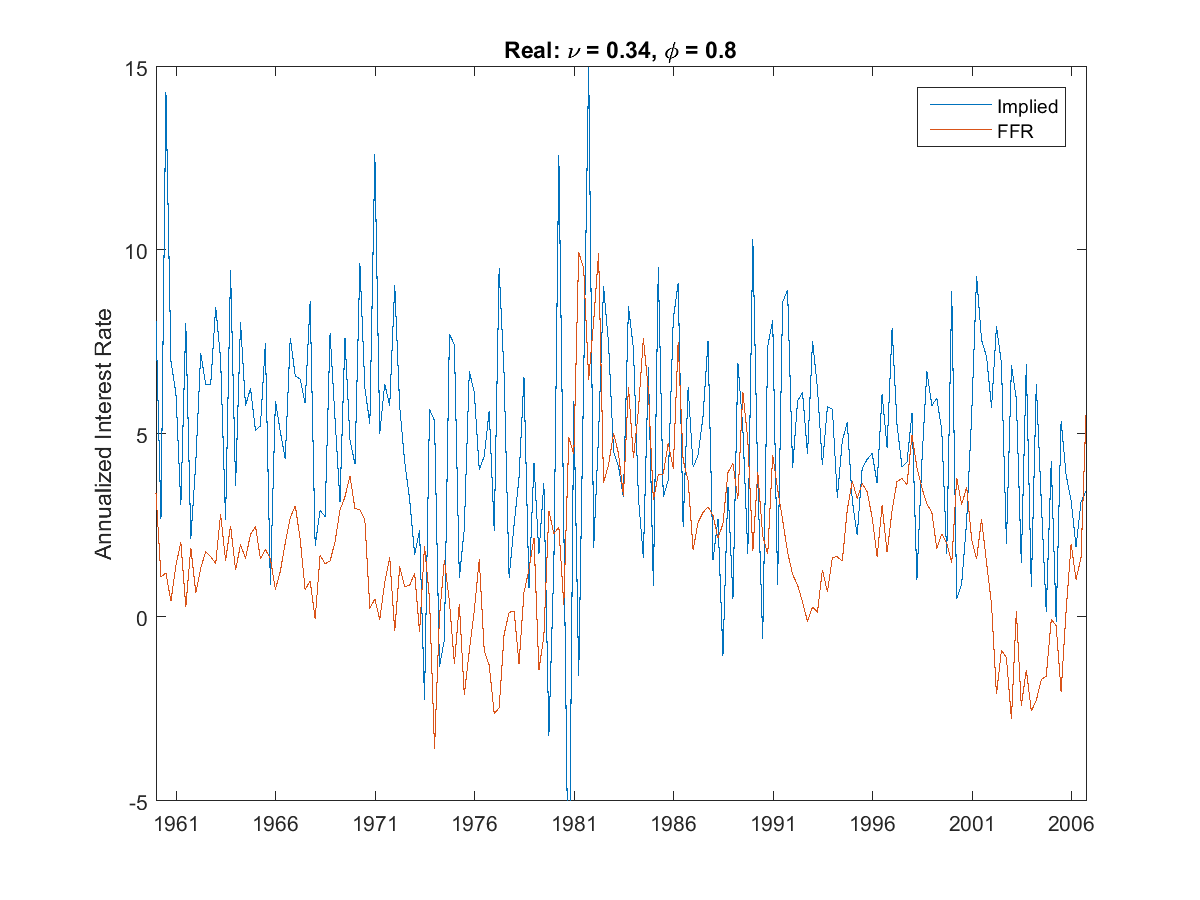
\includegraphics[height=90px]{figs/implied_ffr/real_4.png} \\
\cite{collard11} & Li (2016)
\end{tabular}
\end{center}
\end{frame}

\begin{frame}{Impulse Response}
\begin{itemize}
\item Previously estimated VAR(4)
$$y_t = A_0 + A_1 y_{t-1} + \ldots + A_4 y_{t-4} + \epsilon_t$$
$$\epsilon_t \overset{\text{iid}}{\sim} N(0, \Sigma)$$
\begin{align*}
y_t &= \begin{bmatrix} \log(\text{real consumption}_t) \\ \text{inflation}_t \\ \text{leisure}_t \\ \log(\text{real disposable income}_t) \\ \log(\text{income less consumption}_t) \\ \text{effective FFR}_t \\ \log(\text{CCI}_t) \end{bmatrix}
\end{align*}
\end{itemize}
\end{frame}

\begin{frame}{Impulse Response}
\begin{itemize}
\item Want to observe responses of $y_t$ and implied rate to a $\epsilon_{FFR,0} = 1$ shock to the FFR at $t = 0$
\item Impulse response: $$\frac{\partial y_t}{\partial \epsilon_{FFR,0}} = (A_1^t + A_2^{t-1} + A_3^{t-2} + A_4^{t-3}) \epsilon_0$$
\item Orthogonalized IRF:
  \begin{itemize}
  \item When error terms $\epsilon_{j,t}$ are correlated, exogenous shock to FFR will be correlated with shock to other covariates
  \item Cholesky decomposition $\Sigma = PP'$
  \item New error terms $u_t = P^{-1} \epsilon_t \sim N(0, I)$
  \item Orthogonalized shock $\frac{\partial y_t}{\partial u_{FFR,0}}$
  \end{itemize}
\end{itemize}
\end{frame}

\begin{frame}{Impulse Response}
\begin{itemize}
\item Generate $y_t^\text{no shock}$ for $t = 0, \ldots, 20$ by iterating forward with estimated VAR coefficients from $y_0 = \hat{\mu}$ (sample mean)
\item Using \cite{kilian98}, for each treatment, for 1000 simulations:
  \begin{enumerate}
  \item Simulate data series by choosing random start point $y_0$ and iterating forward with random errors
  \item Compute $\frac{\partial y_t}{\partial u_{FFR,0}}$ for simulated series
  \item Generate $y_t^\text{shock} = y_t^\text{no shock} + \frac{\partial y_t}{\partial u_{FFR,0}}$
  \item Compute implied rates and impulse response using $y_t^\text{no shock}$ and $y_t^\text{shock}$: $$\frac{\partial \log(1+r_t)}{\partial u_{FFR,0}} \approx \log(1 + r_t^\text{shock}) - \log(1 + r_t^\text{no shock})$$
  \end{enumerate}
\item Plot 5th, 50th, and 95th percentiles for each treatment
\end{itemize}
\end{frame}

\begin{frame}{Results: Nominal Rate}
\begin{columns}
\column{0.35\textwidth}
  \centering
  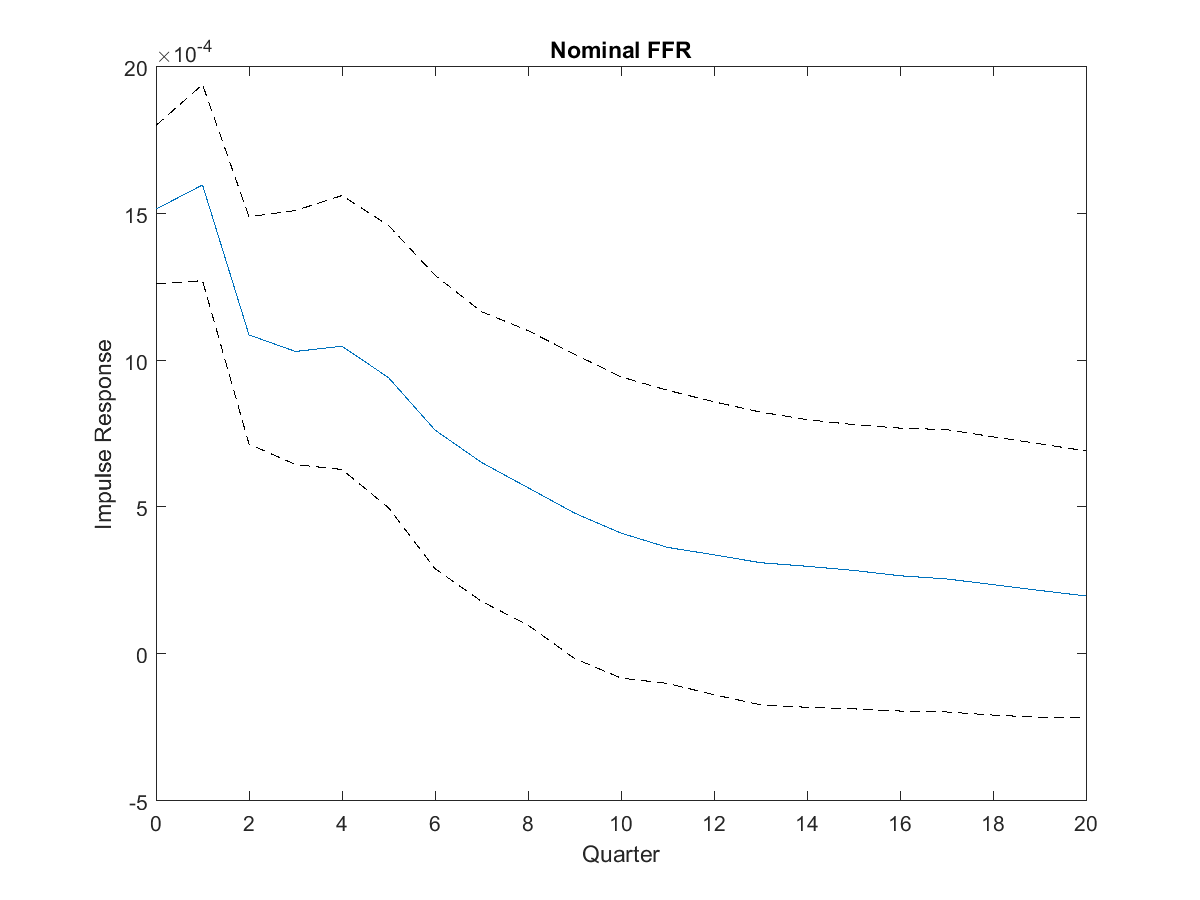
\includegraphics[width=\textwidth]{figs/irf/nominal_ffr.png} \\
  FFR
\column{0.65\textwidth}
  \begin{tabular}{cc}
  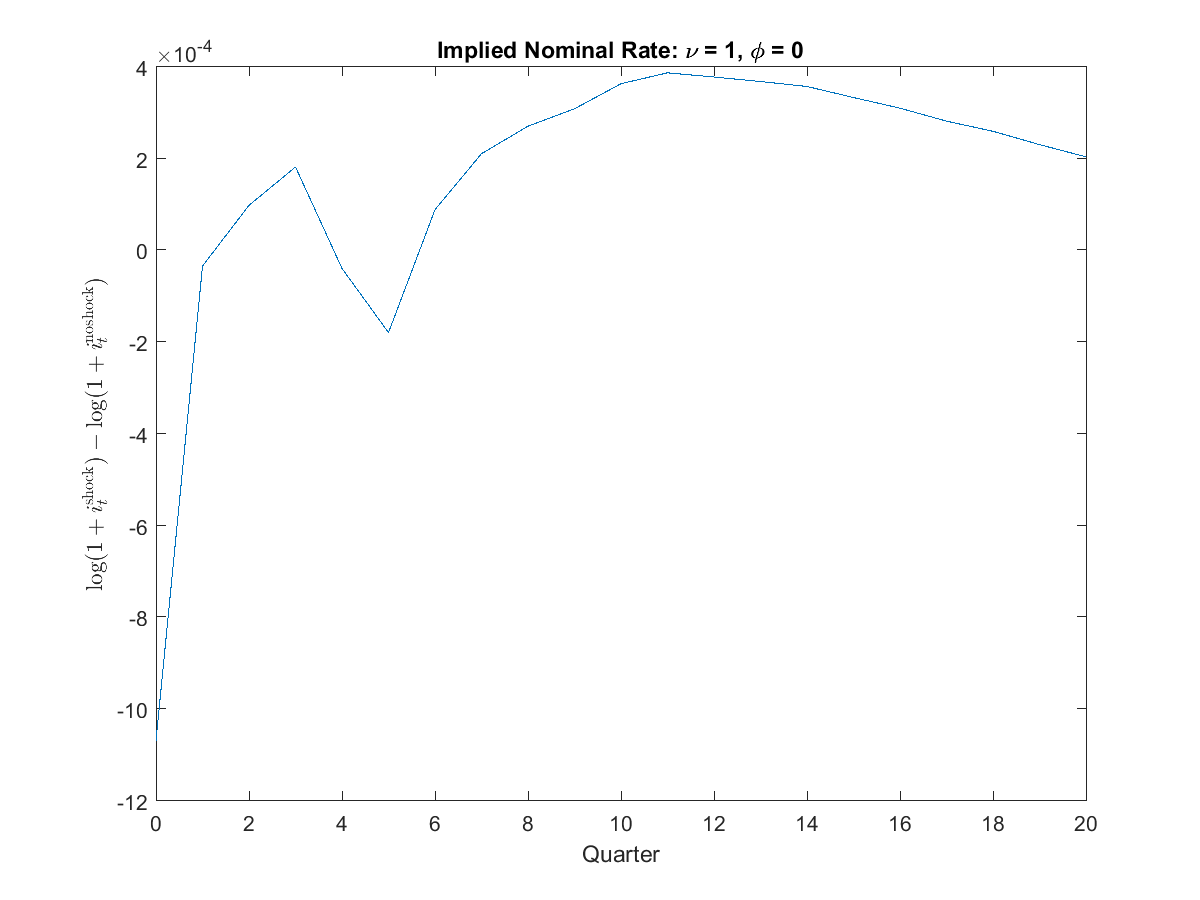
\includegraphics[width=0.45\textwidth]{figs/irf/nominal_implied_1.png} &
  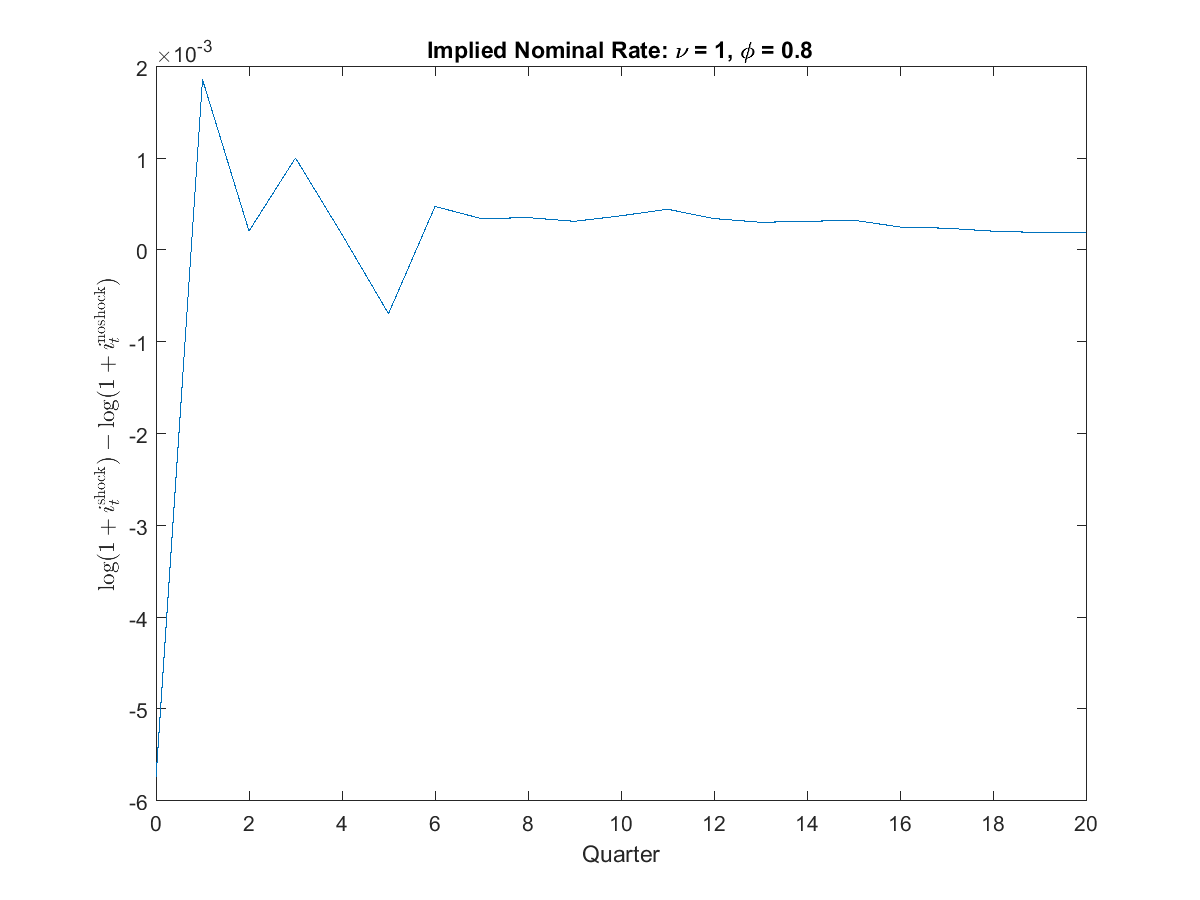
\includegraphics[width=0.45\textwidth]{figs/irf/nominal_implied_2.png} \\
  SEP & SEP + HP \\
  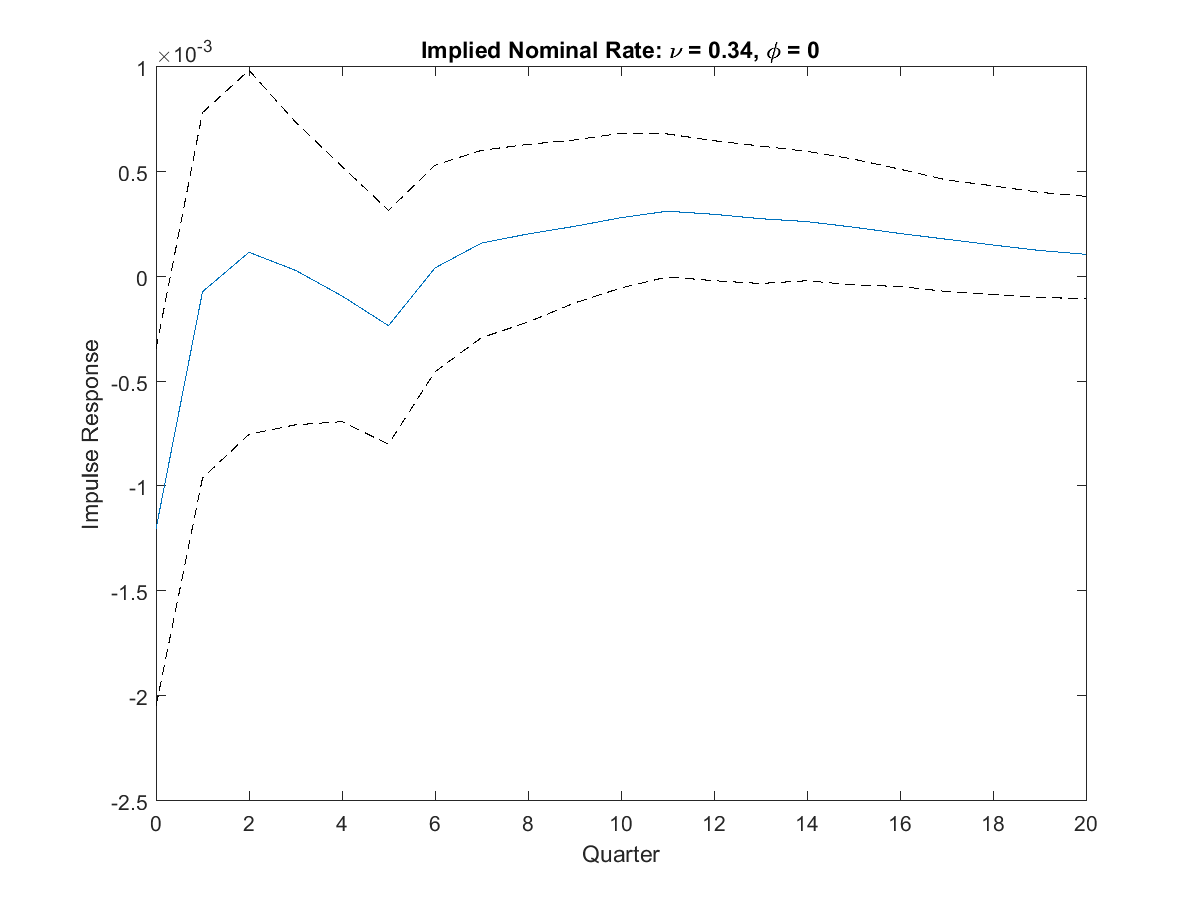
\includegraphics[width=0.45\textwidth]{figs/irf/nominal_implied_3.png} &
  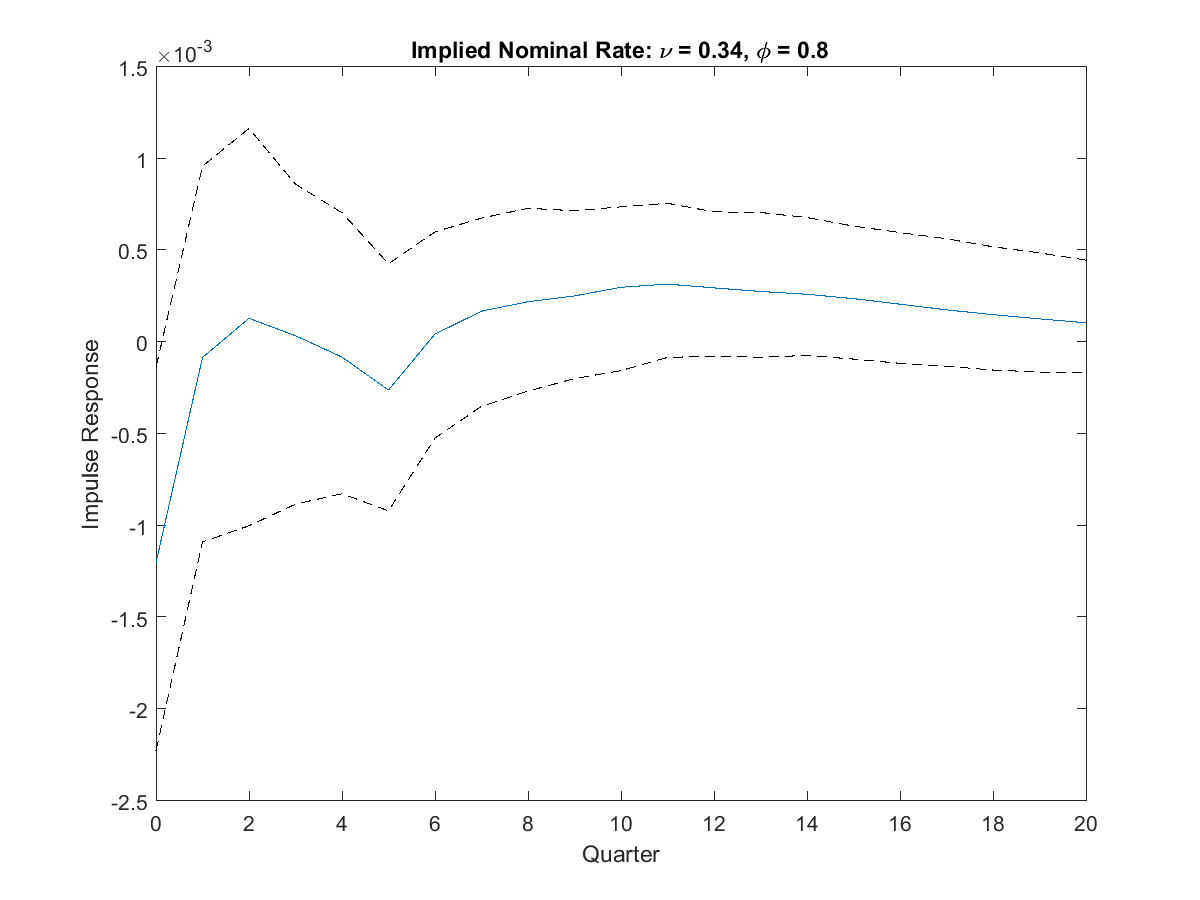
\includegraphics[width=0.45\textwidth]{figs/irf/nominal_implied_4.png} \\
  NSEP & NSEP + HP
\end{tabular}
\end{columns}
\end{frame}

\begin{frame}{Results: Real Rate}
\begin{columns}
\column{0.35\textwidth}
  \centering
  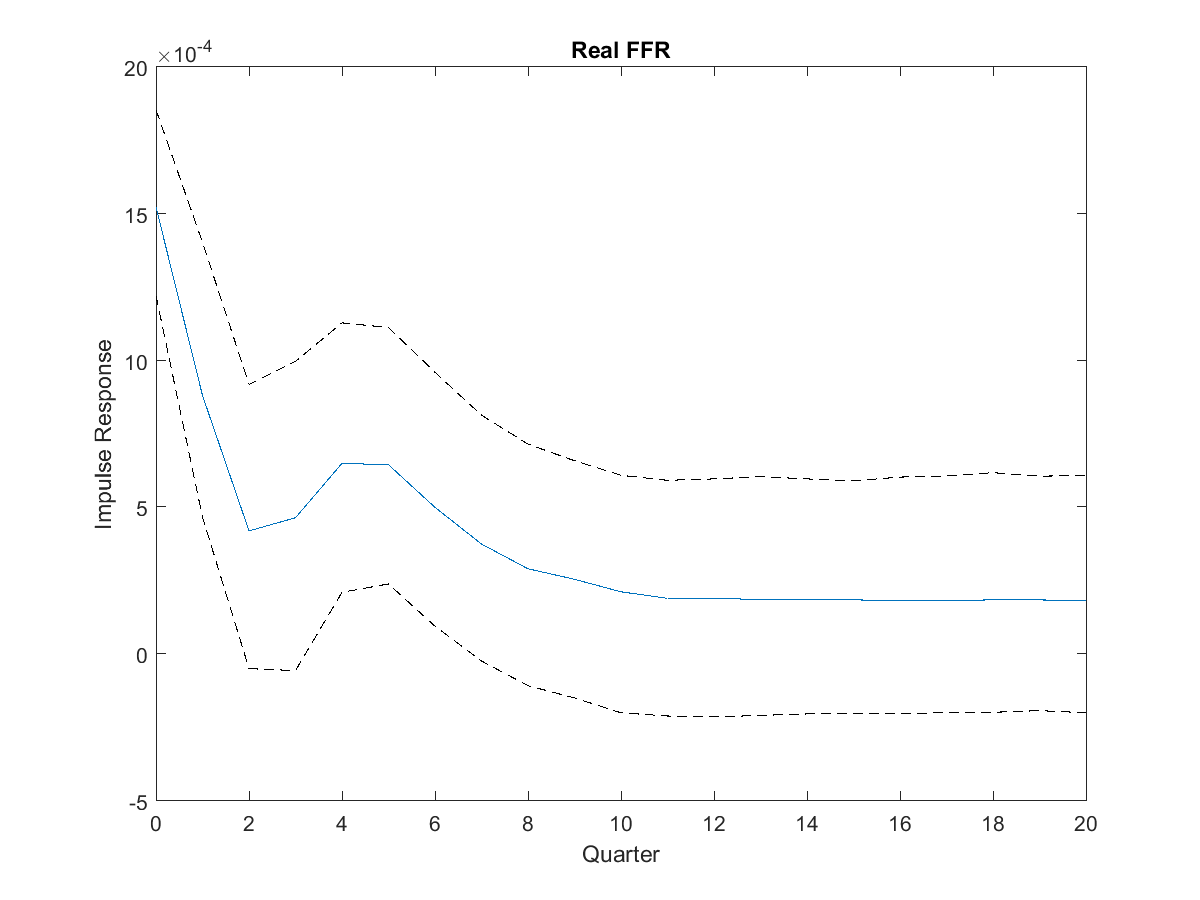
\includegraphics[width=\textwidth]{figs/irf/real_ffr.png} \\
  FFR
\column{0.65\textwidth}
  \begin{tabular}{cc}
  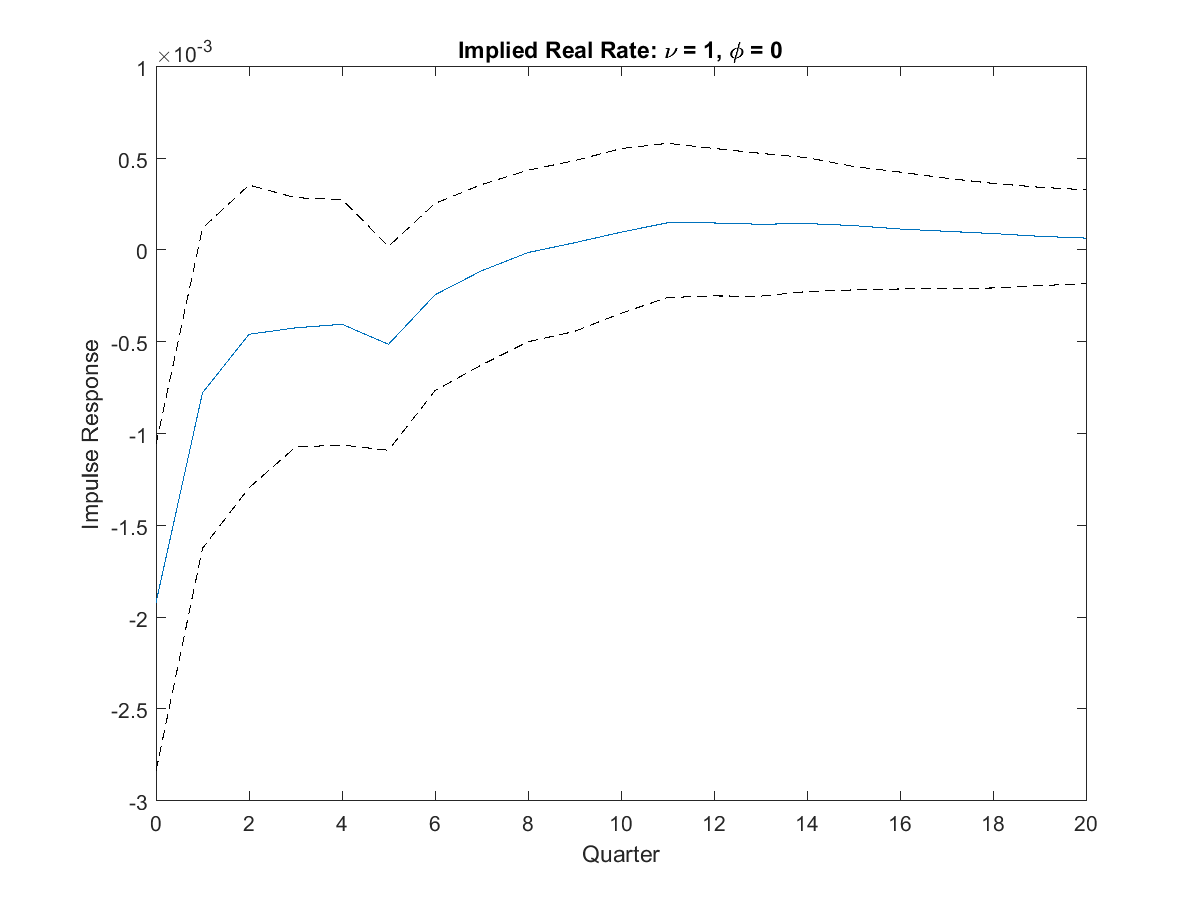
\includegraphics[width=0.45\textwidth]{figs/irf/real_implied_1.png} &
  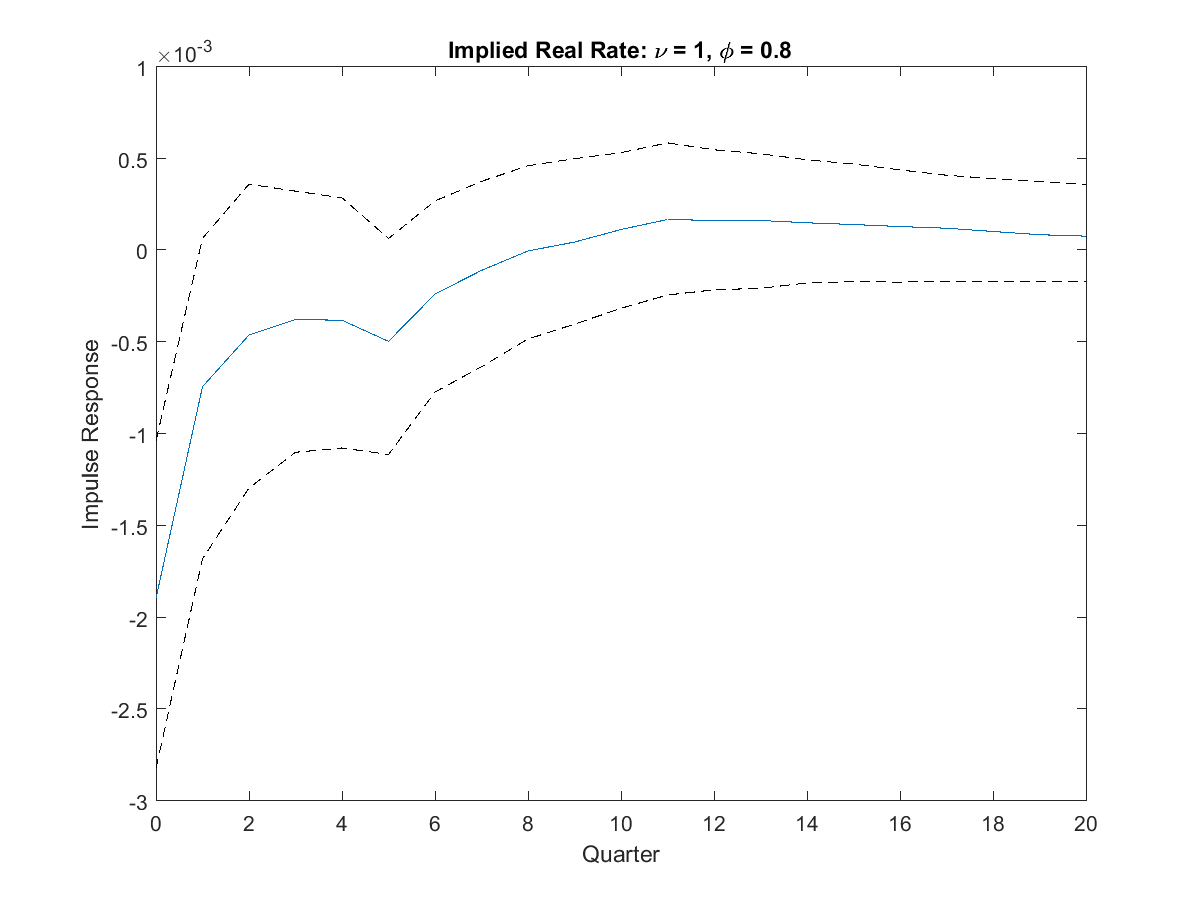
\includegraphics[width=0.45\textwidth]{figs/irf/real_implied_2.png} \\
  SEP & SEP + HP \\
  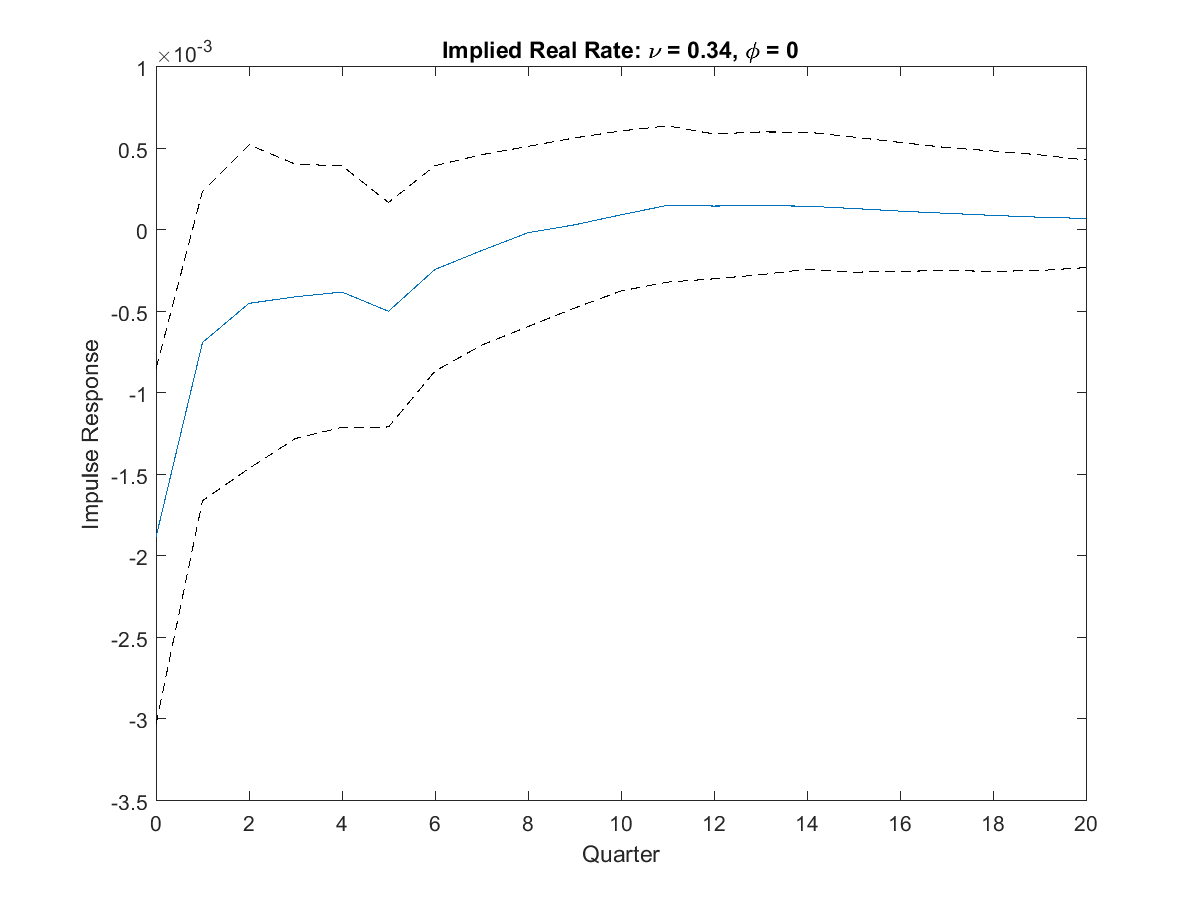
\includegraphics[width=0.45\textwidth]{figs/irf/real_implied_3.png} &
  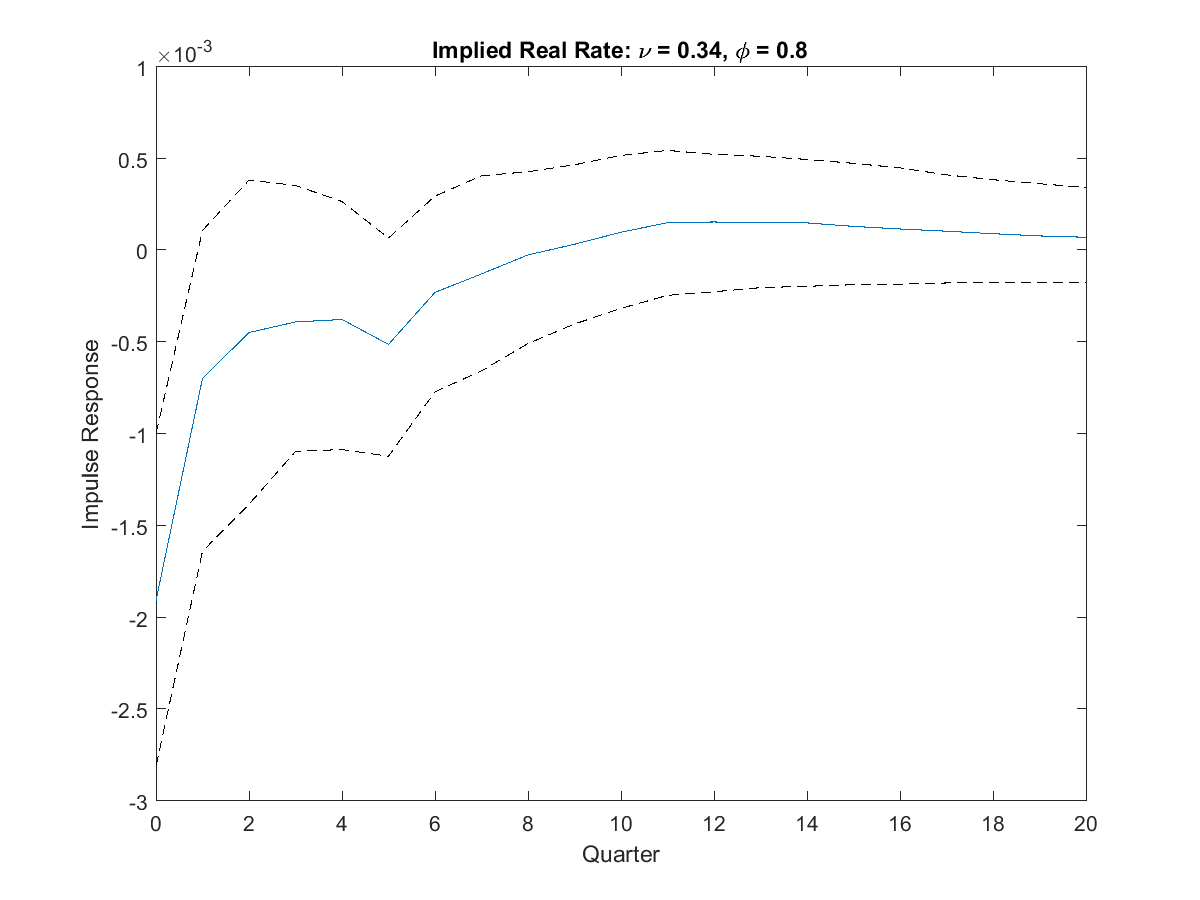
\includegraphics[width=0.45\textwidth]{figs/irf/real_implied_4.png} \\
  NSEP & NSEP + HP
\end{tabular}
\end{columns}
\end{frame}

\againframe<2>{implied_ffr_sep-hp}

\begin{frame}{Problems: SEP + HP Implied Rates}
\begin{itemize}
\item SEP + HP volatility much lower than in \cite{collard11} and \cite{canzoneri07}
  \begin{itemize}
  \item Implied real rates had standard deviation of 6.64 vs. 33.76 and 31.25
  \item SEP + HP still has largest SD of all treatments
  \end{itemize}
\end{itemize}
\end{frame}

\begin{frame}{Problems: NSEP + HP Impulse Response}
\begin{center}
\begin{tabular}{cc}
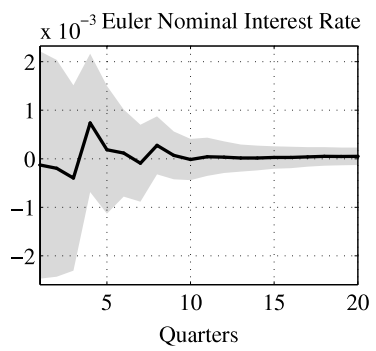
\includegraphics[height=90px]{figs/irf/nominal_implied_4_collard.png} &
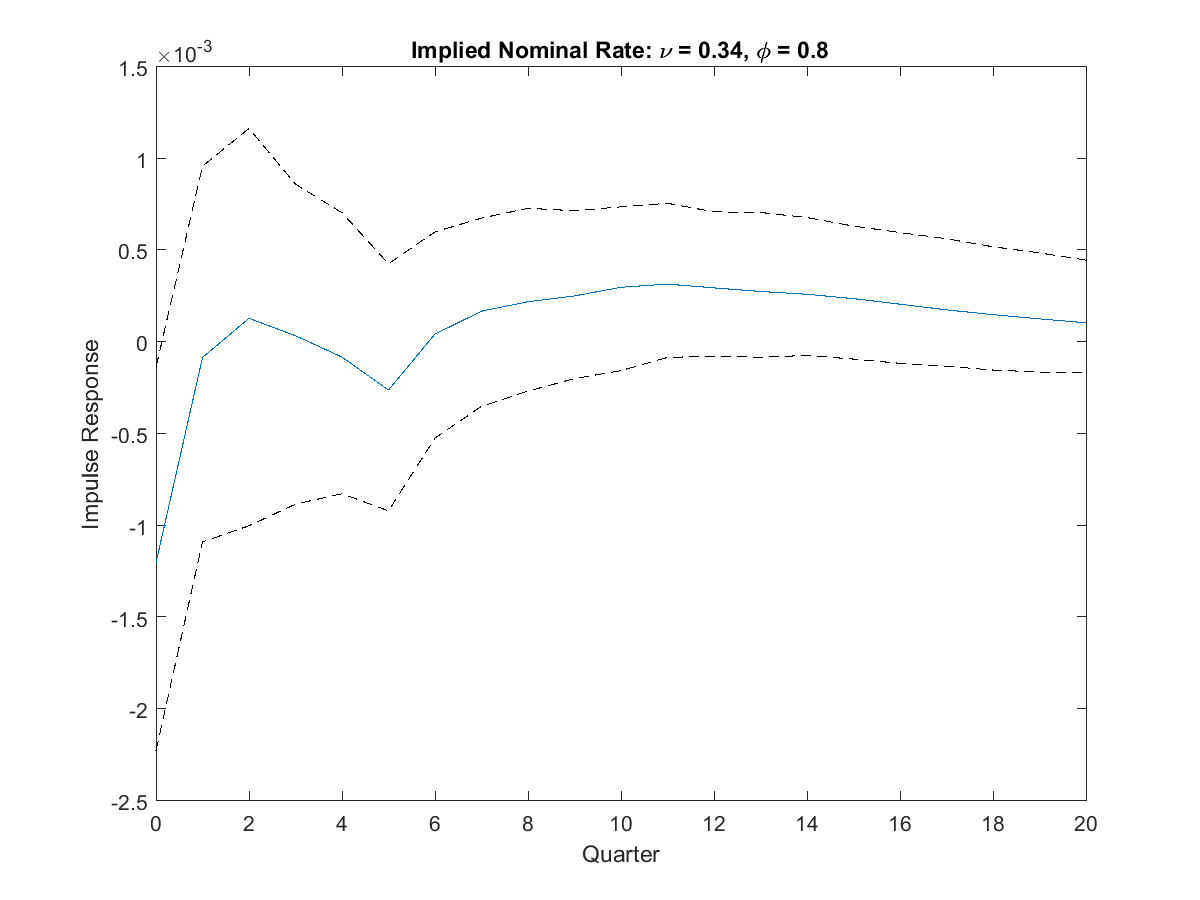
\includegraphics[height=90px]{figs/irf/nominal_implied_4.png} \\
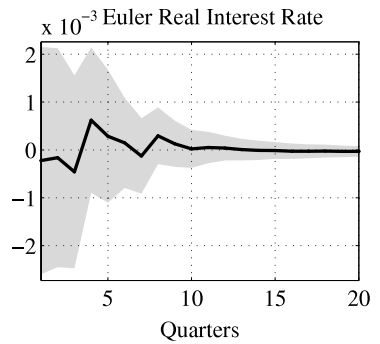
\includegraphics[height=90px]{figs/irf/real_implied_4_collard.png} &
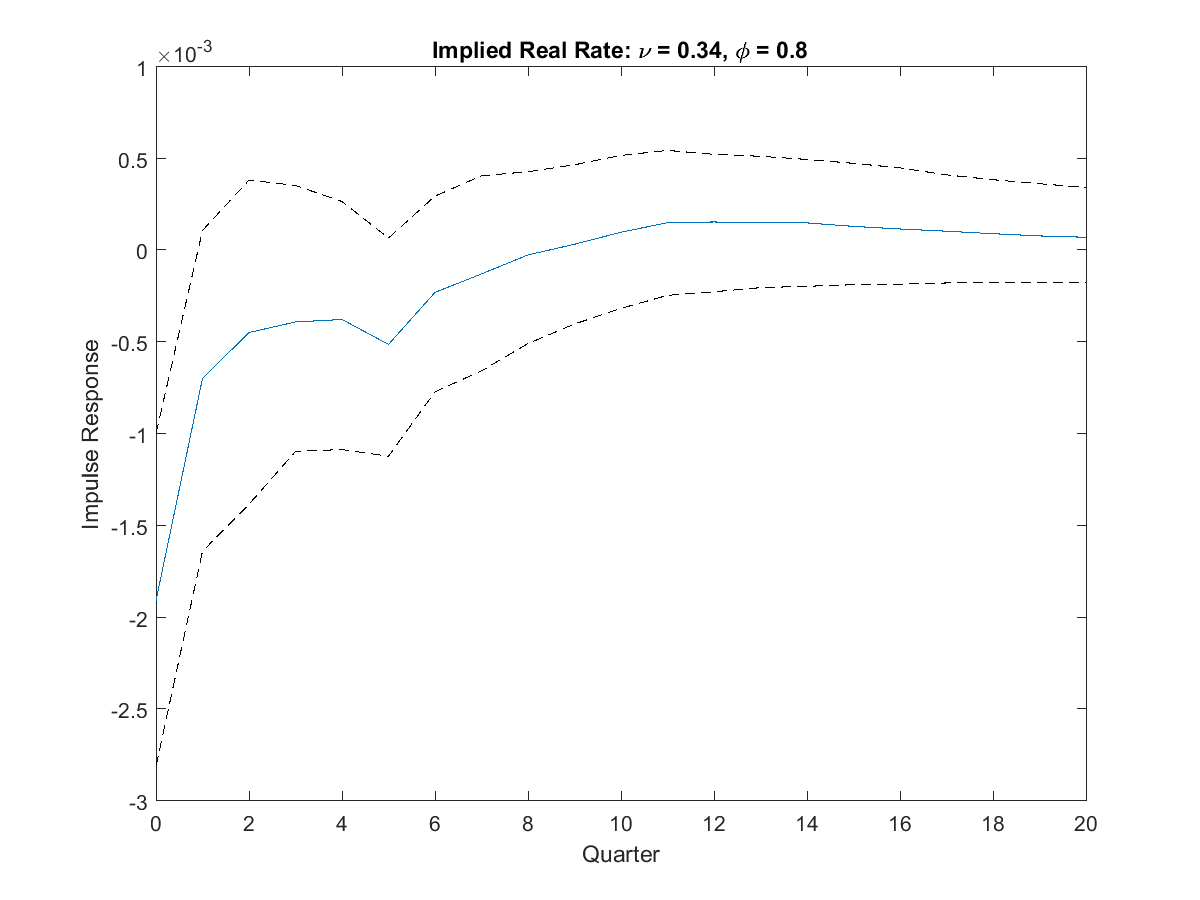
\includegraphics[height=90px]{figs/irf/real_implied_4.png} \\
\cite{collard11} & Li (2016)
\end{tabular}
\end{center}
\end{frame}

\begin{frame}{Other Challenges}
\begin{itemize}
\item Maintaining code modularity and organization
\item No way to export impulse response tables from Stata
\item Computing impulse responses of implied rates (i.e. as a function of $y_t$ impulse response)
\item \cite{kilian98}'s 18-year-old MATLAB code
\end{itemize}
\end{frame}

\begin{frame}{Next}
\begin{itemize}
\item Monte Carlo experiment
\item \textbf{Heterogeneous preferences} (still)
\end{itemize}
\end{frame}

\begin{frame}{References}
\bibliographystyle{../refs/econ}
\bibliography{../refs/refs}
\end{frame}

\end{document}